% =====================================================================
% Nature Climate Change — Article (initial submission, anonymised)
% Compile: pdflatex main && bibtex main && pdflatex main && pdflatex main
% =====================================================================
\documentclass[12pt,a4paper]{article}
\usepackage[margin=2.5cm]{geometry}
\usepackage[T1]{fontenc}
\usepackage[utf8]{inputenc}
\usepackage{lmodern}
\usepackage{graphicx}
\usepackage{booktabs}
\usepackage{amsmath}
\usepackage{xcolor}
\usepackage{setspace}
\usepackage[super,sort&compress]{natbib}
\usepackage[hidelinks]{hyperref}
\usepackage{caption}
\captionsetup{font=small,labelfont=bf}
\graphicspath{{../figures/}{./}}
\setlength{\bibsep}{2pt}
\onehalfspacing
\newcommand{\dd}{\ensuremath{\,^{\circ}\mathrm{C}}}

\title{\textbf{Night-time moist heat driven by humidity, not temperature alone, is crossing
physiologically anchored survival thresholds --- with mortality risk attaching to the crossing
event itself}}

\author{[Author list and affiliations withheld for double-blind peer review]\\[4pt]
\small Initial submission prepared for \textit{Nature Climate Change}.}
\date{}

\begin{document}
\maketitle

\begin{abstract}
\noindent Humid-heat risk assessments rest on daytime, intensity-based indices anchored to a
theoretical 35\,\dd~wet-bulb survival limit that laboratory physiology now shows to be too high.
Using sub-hourly observations from 176 globally distributed stations (1976--2023), we show that
night-time hours above a physiologically anchored 21.9\,\dd~wet-bulb threshold have increased by
$+42.8$ hours per decade, that warming alone explains none of this rise (humidity requirement
$+106\%$), and that climate models overstate the observed rise by $2.3$--$2.9\times$ after optimal
fingerprint scaling. In 225 European regions (77,551 region-weeks), mortality risk attaches to
\emph{crossing} the threshold rather than to its duration, so scaling risk by intensity growth
($+47\%$) instead of extent growth ($+26\%$) overstates burden $1.78\times$. Two wet-tropics
cities provide independent sub-annual replication in which humidity, not dry-bulb heat, carries
the signal. Absolute humid-heat thresholds saturate in the tropics, invalidating percentile-based
warning triggers in $75.6\%$ of European regions.
\end{abstract}

% ----------------------------------------------------------------------
% Introduction (no heading per journal style)
% ----------------------------------------------------------------------
The theoretical wet-bulb temperature ($T_\mathrm{w}$) limit of human survivability, 35\,\dd, has
framed humid-heat risk assessment for over a decade\citep{SherwoodHuber2010}. Empirical physiology,
however, places uncompensable heat stress far below this limit: updated survivability limits
correspond to $T_\mathrm{w}\!\approx\!25.8$--$34.1\,\dd$ for young adults and
$\approx\!21.9$--$33.7\,\dd$ for older adults\citep{Vanos2023}, values that independent laboratory
work continues to validate\citep{Meade2025} and that are already being approached during present-day
heat events\citep{PerkinsKirkpatrick2026}. Observational studies report that extreme humid heat has
more than doubled in frequency since 1979\citep{Raymond2020}, and detection and attribution analyses
find anthropogenic fingerprints in heat-stress indices\citep{Knutson2016}. Yet the epidemiological
record needed to translate these physical trends into health burdens is concentrated in temperate,
high-income settings, leaving the regions with the highest $T_\mathrm{w}$ severely
underrepresented\citep{Sherwood2023} --- a gap we address directly.

Two structural biases follow from this mismatch. First, health-relevant exposure has been measured
with daytime, intensity-based indices: daily maximum $T_\mathrm{w}$ counts\citep{Raymond2020},
gridded $T_\mathrm{w}$ extreme indices\citep{Willett2023,Willett2023PartI}, or wet-bulb globe
temperature (WBGT) products\citep{Brimicombe2023}. Whether night-time hours --- when physiological
recovery from daytime heat is expected\citep{Kim2023,Wu2025} --- are crossing low, physiologically
anchored thresholds has not been quantified globally. Second, exposure metrics differ from the
quantity that health models can validate: the optimal heat-stress metric for mortality modelling
varies by country\citep{Lo2023}, station and reanalysis exposure data yield materially different
risk estimates\citep{Mistry2022}, and time aggregation alone biases heat-mortality burden estimates
by 21.6\% at the weekly scale\citep{Ballester2024}. The joint consequence --- that the metric used
for detection and projection is not the metric whose health relevance can be established --- has
not been examined for humid heat.

Here we close this loop with a single, physiologically anchored exposure metric applied consistently
from global detection to European health attribution to wet-tropics replication. We define
$\mathrm{NWH}_T$ as the annual number of night-time hours (solar elevation $<-0.833^\circ$) with
$T_\mathrm{w}\geq T$, computed from sub-hourly station data (NOAA GHCNh) with $T$ anchored to the
21.9\,\dd~older-adult survivability lower bound\citep{Vanos2023} for the global analysis and to
regionally applicable levels for the wet tropics. We quantify the trend and its attribution, test
whether mortality risk follows the crossing event or its duration, decompose exposure extent versus
intensity, and translate the results into observation-constrained projections, a graded warning
scale, and diagnostics for current World Meteorological Organization/World Health Organization
(WMO/WHO) warning guidance\citep{WMOWHO2015,ISO7243}.

% ----------------------------------------------------------------------
\section*{Results}

\subsection*{Night-time humid-heat burden is rising on every usable threshold}
Night-time hours above 21.9\,\dd~averaged 1,546\,h\,yr$^{-1}$ over 1976--2023 across the 64 stations
with $\geq$90\% window coverage and rose by $+42.84$\,h per decade (Fig.~\ref{fig:fig1}a; station
median $+18.27$, sign-test $p=1.0\times10^{-9}$, $n=67$; population-weighted $+52.13$). The trend is
positive in all eight analysis windows tested ($+27.69$ to $+58.62$\,h per decade; Extended Data
Fig.~\ref{fig:ed1}). The 21.9\,\dd~threshold is the lowest at which the metric remains informative:
17.7\% of station-years are zero and the mean has grown $1.22\times$ from its 1976--85 level, whereas
thresholds above 30\,\dd~are floor-inflated (97.6\% of station-years zero at 30.6\,\dd; 99.9\% at
35\,\dd) and cannot measure trends (Fig.~\ref{fig:fig1}b). This zero-inflation structure is itself a
result: the commonly used survivability framing measures exposure almost exclusively through its
rare, daytime tail, whereas the night-time burden grows on thresholds an order of magnitude closer
to physiological limits.

\subsection*{Humidity, not warming alone, drives the night-time rise}
Counterfactual reconstructions that preserve variability and remove trends separately in temperature
and humidity show that warming alone explains $-6\%$ of the $\mathrm{NWH}_{21.9}$ rise (network-level
S-calibre), whereas humidity change is required for $+106\%$ of it; the station-median decomposition
gives $+52\%$ warming, $+105\%$ humidity and a zero interaction (Fig.~\ref{fig:fig2}a). An
independent decomposition on a different station sample ($n=67$) attributes $4\%$ to temperature,
$39\%$ to humidity and $57\%$ to their interaction. Under every alternative detrending calibre the
humidity requirement remains $41$--$118\%$ (Table~\ref{tab:main}). Subtropical stations carry the
signal (humidity $+48.9$\,h per decade), while equatorial stations show almost no trend because they
are already saturated. Consistently, dry-bulb threshold-crossing hours rose by only $+8.8$\,h per
decade over the same period --- $63\%$ slower than the wet-bulb metric.

\subsection*{An anthropogenic fingerprint that models overstate}
Optimal-fingerprint regression of observed $\mathrm{NWH}_{21.9}$ trends (1976--2014) against CMIP6
historical and natural-only simulations yields a single-signal ALL scaling factor of
$b_\mathrm{ALL}=+0.429\pm0.148$ (90\% CI $[0.186,0.671]$), with the natural-only signal rejected
($b_\mathrm{NAT}=-2.52\pm1.11$); the two-signal fit gives $b_\mathrm{ALL}=+0.348\pm0.168$
(Fig.~\ref{fig:fig2}b). Observed trends exceed internal variability by $3.08\sigma$ in the tropics
and $1.36\sigma$ in the subtropics. Because the ALL response must be scaled down to match
observations, unadjusted CMIP6 models overstate the observed rise by $2.3\times$ (single-signal) to
$2.9\times$ (two-signal) (Fig.~\ref{fig:fig2}c) --- consistent with known humid-heat biases in
CMIP6\citep{Schwingshackl2021}. All projections below are therefore scaled by the fingerprint factor
before impact translation.

\subsection*{Mortality attaches to the crossing event, not to its duration}
In 225 European NUTS2 regions with weekly mortality (77,551 warm-season region-weeks, 2001--2024),
weeks in which nocturnal $T_\mathrm{w}$ crossed 21.9\,\dd~in any hour had a death rate
$1.0181\times$ ($95\%$ CI $[1.0104,1.0258]$, $z=+4.62$) that of non-crossing weeks, with an
attributable fraction of $1.77\%$ $[1.02,2.52]$ (Fig.~\ref{fig:fig3}a). Controlling jointly for
dry-bulb tropical nights \emph{strengthens} the humid-heat association to $1.0292$
$[1.0212,1.0373]$, $z=+7.21$ --- the humidity signal is not a dry-bulb alias. Binning weekly
crossing hours reveals a step-shaped dose--response: risk is elevated for any crossing
(0--2\,h: $1.0156$) and does not increase with additional hours ($>20$\,h: $0.9950$,
$z=-0.37$) (Fig.~\ref{fig:fig3}c). The association is present where the exposure has variance
(southern/humid stratum $1.0036$ per SD, $z=+4.75$) and absent where it does not (northern/cool
$1.0009$, contrast $z=+2.26$, $p=0.024$; Fig.~\ref{fig:fig3}d). Aggregating the same panel annually
attenuates the association by $\sim$93\% (z from $+34.4$ to $+1.1$), extending the aggregation-bias
evidence of \citet{Ballester2024} from the daily-to-weekly to the weekly-to-annual transition.

\subsection*{Extent, not intensity, governs risk --- and intensity-based scaling overstates it}
Between the first and last five years of 2000--2024, the European population exposed to nocturnal
21.9\,\dd~crossings grew by $+26\%$ and the number of exposed regions by $+29\%$, while mean
crossing hours grew faster ($+47\%$; $p=0.0014$) (Fig.~\ref{fig:fig5}a). Because the dose--response
is flat beyond the first crossing, risk follows extent, not intensity: scaling burden by the
intensity trend overstates the risk-relevant growth by a factor of $1.78$. Under
observation-constrained SSP2-4.5 and SSP5-8.5 warming, the newly exposed European population reaches
$+78$ and $+146$ million by end-century (unscaled: $+166$ and $+237$ million)
(Fig.~\ref{fig:fig5}b), and each $+1\,\dd$ of warm-season night-time $T_\mathrm{w}$ adds
$42.3$--$70.0$ million people newly exposed (region fixed-effect to pooled logistic dose--response;
Fig.~\ref{fig:fig5}c). The model is calibrated to within $-2.7\%$ of the observed mean.

\subsection*{Wet-tropics replication, threshold failure and the power diagnosis}
Two wet-tropics cities with sub-annual mortality --- Hong Kong (132 warm-season months) and
Singapore (264 months) --- provide the independent replication that the literature
lacks\citep{Sherwood2023}. Monthly $\mathrm{NWH}_{25}$ is associated with mortality in each city
(Hong Kong $1.0140$ per SD, $z=+2.31$; Singapore $1.0073$, $z=+1.69$) and in a random-effects
meta-analysis of the dry-bulb-orthogonalised exposures ($1.0030$ $[1.0009,1.0051]$, $z=+2.83$,
$p=0.0046$, $I^2=0\%$; Fig.~\ref{fig:fig4}a). A pre-specified negative control confirms the
mechanism: the orthogonalised dry-bulb hot-night series carries \emph{no} positive signal (Hong Kong
$z=-2.57$, inverse; Singapore $z=+1.09$) --- in these cities humidity, not dry-bulb heat, carries
the mortality signal.

The same cities demonstrate why globally uniform thresholds fail in the tropics. In Singapore, the
median monthly exceedance fraction is 1.000 at 21.9\,\dd~and 0.981 at 24\,\dd: the exposure
degenerates into night length, and an $\mathrm{NWH}_{21.9}$ mortality model returns a spurious
$z=+8.61$ that we reject as a saturation artefact (Fig.~\ref{fig:fig4}b,c). Re-thresholding restores
validity ($\mathrm{NWH}_{25.0}$: $1.0122$, $z=+2.03$). A power diagnostic explains the long-standing
absence of wet-tropics mortality evidence: Singapore's warm-season night-time $T_\mathrm{w}$ varies
by only $0.50\,\dd$ (SD) against Hong Kong's $1.62\,\dd$, so detecting the same per-degree effect
requires $2.33\times$ larger true effect sizes (minimum detectable effects $1.05$ vs $2.45\%$ per
\dd; Fig.~\ref{fig:fig4}d). The humid-heat evidence gap in the tropics is thus a quantifiable
statistical-power problem, not evidence of absence.

\subsection*{Operational translation and a failure mode of current guidance}
A three-level graded scale built on nocturnal $T_\mathrm{w}$ levels of 21.9, 24 and 25.8\,\dd~is
strictly monotonic in mortality across 225 European regions (level~I $1.0591$
$[1.0384,1.0803]$, $z=+5.68$; level~III $1.2686$ $[1.1183,1.4391]$, $z=+3.70$; trend $1.0577$ per
level, $z=+5.30$; Extended Data Fig.~\ref{fig:ed3}), and in the wet tropics must be replaced by
local quantiles because absolute levels saturate. As a warning layer, the nocturnal trigger alone
detects fewer event weeks than the current daytime rule (POD $0.102$ vs $0.184$) and is therefore
positioned as an \emph{add-on}: it flags 3,142 weeks that the daytime rule misses, with an event
rate $1.53\times$ the panel average. More consequentially, the WMO/WHO default of percentile-based
triggers fails structurally under zero inflation: the 95th percentile of warm-season
$\mathrm{NWH}_{21.9}$ equals zero in $75.6\%$ of European regions ($63.6\%$ at P97.5, $52.4\%$ at
P99) (Extended Data Fig.~\ref{fig:ed4}), so percentile rules cannot fire where they are most needed.
Reference re-implementation at the two cities bounds the combined implementation uncertainty of the
metric at $u_c=35.7$--$39.0\%$, dominated (22--32\%) by the night definition, with wet-bulb formula
choice contributing $<0.6\%$ (Extended Data Fig.~\ref{fig:ed2}); the widely used one-third-rule
approximation biases $\mathrm{NWH}_{25}$ by $+12.1\%$ and must not be used.

% ----------------------------------------------------------------------
\section*{Discussion}
Three findings reorganise how humid-heat health risk should be measured. First, night-time
threshold crossings --- not daytime intensity --- are where the physiologically relevant humid-heat
signal has grown, and humidity change, not warming alone, is its driver. The metric family used in
prior global assessments\citep{Raymond2020,Willett2023,Coffel2018,Tuholske2021} counts rare daytime
extremes; the same stations show the burden shifting into the night on thresholds within the
experimentally validated survivability range\citep{Vanos2023,Meade2025}. Second, mortality risk in
Europe attaches to the crossing event itself. This occurrence-type response conflicts with the
adaptive-threshold behaviour reported for East Asian nighttime-only heatwaves, where risk rises
only at high cumulative intensity\citep{Liu2025}; the distinction is metric-based --- cumulative
excess heat versus physiological threshold crossing --- and population- and scale-based, and it is
directly falsifiable in cohorts with individual-level exposure. Third, because risk follows extent
rather than intensity, impact assessments that scale burden by intensity trends overstate
risk-relevant growth by $1.78\times$ here; the correction is arithmetic, portable, and large.

Our results sharpen rather than soften the caveats. The wet-tropics replication rests on two
high-income, high-adaptation cities; the power diagnosis quantifies why broader tropical evidence is
absent but does not substitute for it. The full-sample exposure--response gradient across Europe is
positive but is driven by regions whose exposure has no variance; restricted to informative regions
the per-unit gradient is negative, consistent with adaptation along the humid-heat gradient
(Extended Data Fig.~\ref{fig:ed5}). Heterogeneity across European regions is substantial
($I^2=78\%$), the fixed-effect per-degree exposure response ($42.3$ million per $+1\,\dd$) should be
treated as the conservative bound, and implementation uncertainty of $36$--$39\%$ is dominated by
the night definition --- arguing for a standardised astronomical definition in future monitoring
(Extended Data Fig.~\ref{fig:ed6}). The annual-aggregation diagnostic extends known aggregation
biases\citep{Ballester2024} and reinforces that sub-annual mortality data are a prerequisite for
humid-heat health assessment. Finally, the structural failure of percentile triggers under zero
inflation is a direct, actionable input for revision of WMO/WHO warning guidance\citep{WMOWHO2015}
and WBGT-based standards\citep{ISO7243,Brimicombe2023}: thresholds in hot-humid regions must be
locally anchored, and the graded scale validated here provides that anchoring while remaining
monotonic in mortality.

The observation-constrained projections --- $42$--$70$ million Europeans newly exposed per
$+1\,\dd$ of night-time humid heat, and $+78$ to $+146$ million by end-century under SSP2-4.5 and
SSP5-8.5 --- translate a physiologically anchored metric into policy-relevant numbers with the model
bias removed rather than inherited\citep{IPCCAR6Ch11,Coffel2018}. Given that exposure metrics, not
emissions scenarios, dominate the spread in heat-stress impact projections\citep{Schwingshackl2021},
adopting crossing-based, night-limited, locally anchored metrics is the single most consequential
methodological change available to humid-heat impact assessment.

% ----------------------------------------------------------------------
\section*{Methods}
\subsection*{Data}
Night-time exposure is computed from NOAA GHCNh sub-hourly station records (version 1.1.0):
176 stations with $\geq$20 qualifying station-years yield 4,164 of 4,763 downloaded station-years
(87\%) after quality control; 67 stations enter headline panels ($n=64$ for the balanced
1976--2023 network-mean series). Station populations use GeoNames city points within 50\,km with
exponential decay to 300\,km (9.01 billion person-equivalents of coverage). European weekly deaths
are Eurostat NUTS3 weekly counts aggregated to 2021 NUTS2 (225 regions); gridded exposure uses NASA
POWER (MERRA-2) with an Open-Meteo/ERA5 cross-check. City panels use Hong Kong Census and Statistics
monthly deaths (Table 115-01022A) and Singapore SingStat registered deaths (M810121) with NASA POWER
hourly meteorology. CMIP6 historical, SSP2-4.5, SSP5-8.5, DAMIP natural-only and piControl runs
(tasmin, hurs) from five models (CNRM-CM6-1, CanESM5, HadGEM3-GC31-LL, IPSL-CM6A-LR, MRI-ESM2-0)
follow \citet{Eyring2016}. External validation uses HadEX3 TN90p and GISTEMP v4. WHO Mortality
Database annual panels were used only for negative diagnostics and are reported in the
Supplementary Information. Humidity's role in heat--health outcomes remains debated in the
epidemiological literature\citep{Baldwin2023}; distributed-lag and nonlinear exposure--response
conventions follow \citet{GasparriniDLNM2011}.

\subsection*{Wet-bulb temperature and the NWH metric}
$T_\mathrm{w}$ is computed per hourly record from dry-bulb temperature and dew point by iterative
solution of the psychrometric equation (Stull and Davies-Jones implementations cross-validated to
$0.05\,\dd$; dew-point inversion as reference). Night is defined by solar elevation
$<-0.833^\circ$ computed from station coordinates, not by clock hour, because station timestamps
are UTC. $\mathrm{NWH}_T$ counts night-time hours with $T_\mathrm{w}\geq T$ per station-year.
Thresholds: 21.9\,\dd~(older-adult survivability lower bound\citep{Vanos2023}) as headline; 23, 24,
25.8, 30.6 and 35\,\dd~as the ladder; 25.0 and 25.8\,\dd~for wet-tropics city models.

\subsection*{Trends, uncertainty and homogeneity}
Trends use Theil--Sen regression with Mann--Kendall tests and Benjamini--Hochberg false-discovery
control; spatial dependence is handled via Bretherton effective sample sizes and spherical
$k$-means cluster bootstrap (headline 95\% CI for the station-median trend $[+3.4,+57.0]$\,h per
decade). Relative homogeneity uses up to five reference neighbours within 1,500\,km with Pettitt
changepoint screening; homogenisation changes the trend ratio by $1.00$. Urban-heat-island
contamination is bounded by the most-rural quartile remaining significant ($p=6.8\times10^{-4}$).
Independent confirmation: HadEX3 TN90p versus night-recovery failure rate $r=0.402$
($p=0.0069$; 92\% sign agreement among non-zero stations).

\subsection*{Humidity necessity decomposition}
Counterfactual series A (observed), B (temperature detrended), C (humidity detrended) and D (both
detrended) are built with variance-preserving LOWESS detrending (S-calibre). Main effects are
referenced to D: temperature $=\mathrm{tr}(B)-\mathrm{tr}(D)$, humidity
$=\mathrm{tr}(C)-\mathrm{tr}(D)$, interaction
$=\mathrm{tr}(A)-\mathrm{tr}(B)-\mathrm{tr}(C)+\mathrm{tr}(D)$. Network-aggregated (equal-weight
annual means) and station-median variants are reported; linear and climatology-locked calibres are
shown as sensitivities.

\subsection*{Detection and attribution}
Optimal-fingerprint total-least-squares regression of the two-dimensional (tropical, subtropical)
observed trend vector on ALL and NAT ensemble-mean responses, with noise covariance from 67
non-overlapping 39-year piControl segments; 90\% confidence intervals are profiled. Projections are
scaled by $b_\mathrm{ALL}$ (single signal) before impact translation; the transfer function from
monthly mean/SD to crossing hours is validated against observed annual $\mathrm{NWH}$
($R^2=0.9992$, bias $+0.2$\,h\,yr$^{-1}$).

\subsection*{European health panel}
Poisson generalised linear models with region and year fixed effects, Fourier seasonality (weekly),
and region-clustered robust standard errors; exposures are raw binary (any nocturnal hour
$\geq21.9\,\dd$), z-standardised continuous hours, or joint dry-bulb controls (tropical night, TX
$\geq30\,\dd$). Regional estimates are pooled by DerSimonian--Laird random effects with
empirical-Bayes shrinkage; heterogeneity is $I^2=78.2\%$ and is reported with the region-level
effect distribution (median $1.021$; $74.3\%$ of regions $>1$). Lag-1 displacement is null
($0.9979$), excluding harvesting. Gradient analyses regress regional slopes on background nocturnal
$T_\mathrm{w}$ with cluster bootstrap, restricted and unrestricted (Extended Data
Fig.~\ref{fig:ed5}).

\subsection*{Wet-tropics city panels and power}
Monthly Poisson models with year splines (df 8), bimonthly Fourier terms, raw and
dry-bulb-orthogonalised exposures; meta-analysis via random effects. Minimum detectable effects
convert 80\%-power detectable rate ratios per SD into per-degree equivalents. Negative control:
orthogonalised dry-bulb hot nights ($\geq28\,\dd$).

\subsection*{Exposure extent, intensity and projections}
Extent (share of population/regions with any crossing) and intensity (mean crossing hours) are
compared over first-versus-last five-year means (2000--2024, 135 regions, 499 million people).
The dose--response mapping uses a pooled logistic model calibrated to the observed mean, with a
region fixed-effect alternative; scenario warming (CMIP6 multi-model mean, fingerprint-scaled) is
applied to the fitted response.

\subsection*{Grading, warning skill and implementation uncertainty}
The graded scale assigns European region-weeks to levels I--III by nocturnal $T_\mathrm{w}$
thresholds (21.9/24/25.8\,\dd) and evaluates monotonicity in the same Poisson framework;
wet-tropics versions use within-city quantiles (cluster-robust SEs are unreliable with two clusters
and are reported with HC0 intervals). Warning skill (POD, FAR, Heidke) compares four triggers on
the same panel. Implementation uncertainty combines wet-bulb formula, night definition, input and
instrument terms by root-sum-square from a reference re-implementation at both cities.

\subsection*{Code}
All analyses are Python 3.13 (statsmodels, numpy, scipy, xarray). The full pipeline (steps
1--54), frozen result artefacts with SHA-256 hashes, and one-command reproduction of every figure
and number in this Article are publicly available at
\url{https://github.com/fanqimcse/nocturnal-moist-heat-burden} (tag v1.0.0; archival request
accepted by Software Heritage; a DOI will be minted on acceptance).

\section*{Data availability}
NOAA Global Historical Climatology Network-hourly (GHCNh) v1.1.0 (NCEI, https://www.ncei.noaa.gov);
Eurostat weekly death statistics (https://ec.europa.eu/eurostat); NASA POWER
(https://power.larc.nasa.gov); Open-Meteo ERA5 archive (https://open-meteo.com); Hong Kong Census
and Statistics Department Table 115-01022A (https://www.censtatd.gov.hk); Singapore Department of
Statistics M810121 (https://www.singstat.gov.sg); CMIP6 via the Earth System Grid Federation
(https://esgf-node.llnl.gov); HadEX3 (https://www.climdex.org); GISTEMP v4
(https://data.giss.nasa.gov/gistemp); GeoNames (https://www.geonames.org); WHO Mortality Database
(https://www.who.int/data/gho/data/themes/mortality-and-global-health-estimates). All datasets are
public; no new empirical data were collected.

\section*{Code availability}
The analysis pipeline, frozen artefacts (SHA-256 indexed), figure-generation code
(\texttt{make\_figures.py}) and a reproduction script for every reported number are available at
the repository above and accompany the submission as Supplementary Software.

% ----------------------------------------------------------------------
\begingroup
\renewcommand{\bibsection}{\section*{References}}
\bibliographystyle{unsrtnat}
\bibliography{references}
\endgroup

\clearpage
% ---------------------------------------------------------------------
% captions.tex — main figure captions, main table, Extended Data captions
% ---------------------------------------------------------------------
\section*{Main figures and table}

\begin{figure}[htbp]
\centering
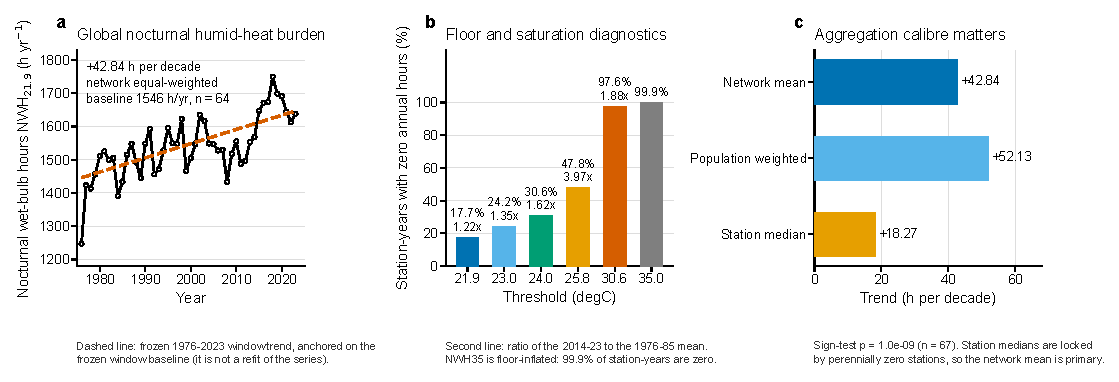
\includegraphics[width=\textwidth]{Fig1.pdf}
\caption{\textbf{Global night-time humid-heat burden and the choice of threshold.}
\textbf{a}, Annual network-mean night-time hours with wet-bulb temperature $\geq21.9$\,\dd{}
($\mathrm{NWH}_{21.9}$), 1976--2023, 64 stations with $\geq$90\% window coverage; dashed line is
the frozen window trend ($+42.84$\,h per decade) anchored on the 1976--85 baseline
(1,546\,h\,yr$^{-1}$). \textbf{b}, Zero-inflation diagnostic: share of station-years with zero
crossing hours (bars) and growth ratio of 2014--23 to 1976--85 means (labels) by threshold;
thresholds above 30\,\dd{} are floor-inflated. \textbf{c}, Aggregation calibre matters: network
mean ($+42.84$), population-weighted ($+52.13$) and station median ($+18.27$) trends on the
identical station set; the station median is locked by permanently zero stations, so the network
mean is primary.}
\label{fig:fig1}
\end{figure}

\begin{figure}[htbp]
\centering
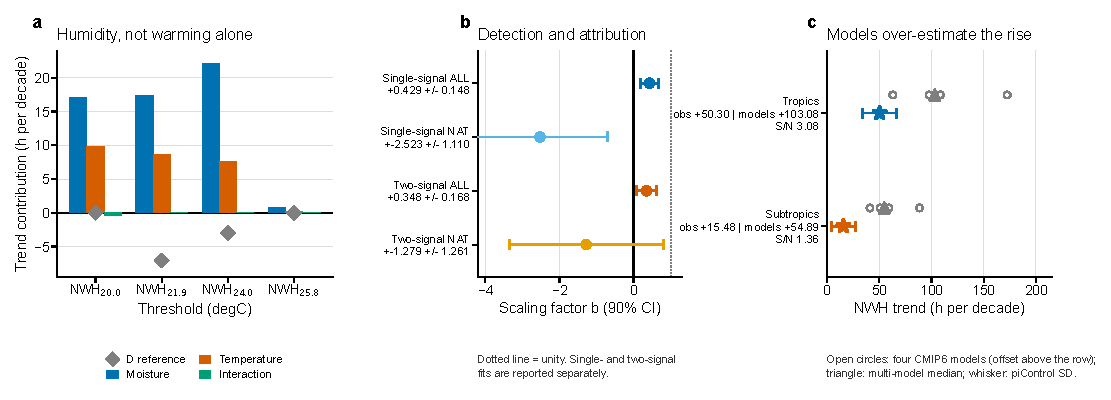
\includegraphics[width=\textwidth]{Fig2.pdf}
\caption{\textbf{Humidity necessity and anthropogenic detection.}
\textbf{a}, Variance-preserving counterfactual decomposition of the $\mathrm{NWH}_{21.9}$ trend by
threshold (station-median calibre, $n=72$): moisture (blue), temperature (orange), interaction
(green), double-detrended reference (diamond). \textbf{b}, Optimal-fingerprint scaling factors with
90\% confidence intervals: single-signal ALL ($+0.429\pm0.148$), single-signal NAT (rejected),
two-signal ALL ($+0.348\pm0.168$) and two-signal NAT. \textbf{c}, Observed versus CMIP6
$\mathrm{NWH}$ trends (h per decade): open circles, individual models; triangles, multi-model
median; whisker, piControl internal variability; observation-to-internal-variability ratios 3.08
(tropics) and 1.36 (subtropics).}
\label{fig:fig2}
\end{figure}

\begin{figure}[htbp]
\centering
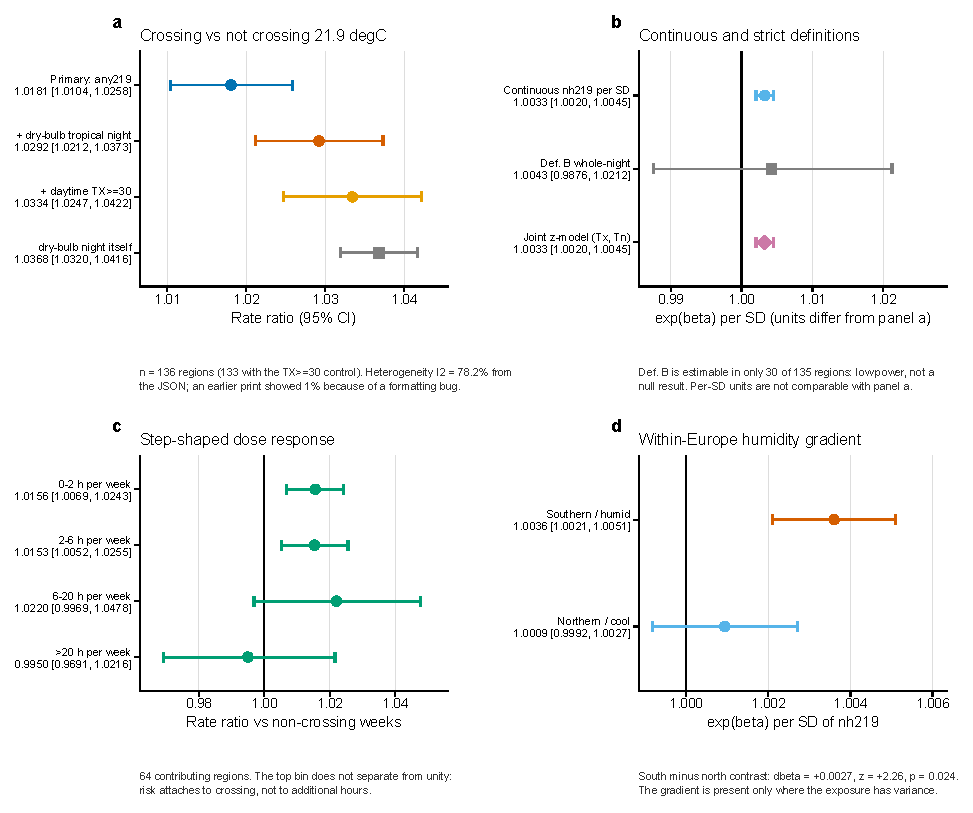
\includegraphics[width=\textwidth]{Fig3.pdf}
\caption{\textbf{Mortality attaches to the crossing event (Europe, weekly, 2001--2024).}
\textbf{a}, Rate ratios for weeks with any nocturnal hour $\geq21.9$\,\dd{}, alone and adjusted for
dry-bulb tropical nights or daytime TX $\geq30$\,\dd{} (136 regions; 133 with the TX control).
\textbf{b}, Continuous (per SD) and strict whole-night definitions; definition B is estimable in
only 30 regions (low power, not a null result). \textbf{c}, Dose--response by weekly crossing
hours: risk attaches to the first crossing and does not increase with additional hours.
\textbf{d}, Southern/humid versus northern/cool strata (per SD of continuous exposure); contrast
$z=+2.26$, $p=0.024$.}
\label{fig:fig3}
\end{figure}

\begin{figure}[htbp]
\centering
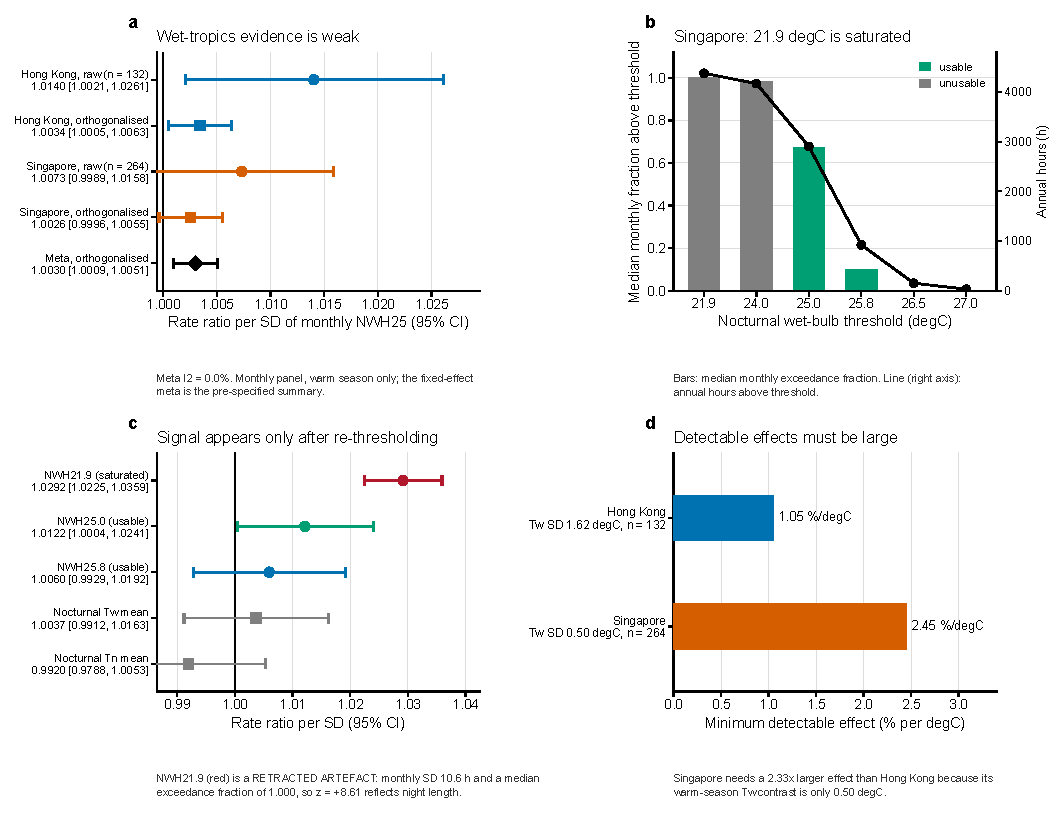
\includegraphics[width=\textwidth]{Fig4.pdf}
\caption{\textbf{Wet-tropics replication, threshold failure and statistical power.}
\textbf{a}, Monthly $\mathrm{NWH}_{25}$ mortality associations (rate ratio per SD, 95\% CI) for
Hong Kong ($n=132$ months) and Singapore ($n=264$), raw and dry-bulb-orthogonalised, with the
pre-specified random-effects meta-analysis ($I^2=0\%$). \textbf{b}, Singapore threshold
saturation: median monthly exceedance fraction (bars; usable in green) and annual crossing hours
(line, right axis); 21.9 and 24\,\dd{} are saturated. \textbf{c}, Re-thresholded models: the
$\mathrm{NWH}_{21.9}$ result (red) is a rejected saturation artefact (median exceedance fraction
1.000; $z=+8.61$ reflects night length); 25.0 and 25.8\,\dd{} are valid. \textbf{d}, Minimum
detectable effects: Singapore requires a $2.33\times$ larger true effect than Hong Kong because its
warm-season night-time $T_\mathrm{w}$ varies by only 0.50\,\dd{} (SD) versus 1.62\,\dd{}.}
\label{fig:fig4}
\end{figure}

\begin{figure}[htbp]
\centering
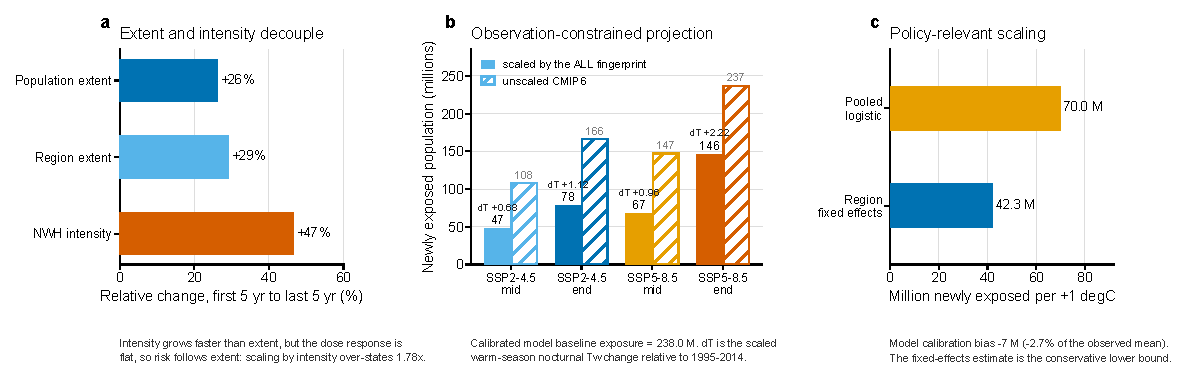
\includegraphics[width=\textwidth]{Fig5.pdf}
\caption{\textbf{Extent--intensity decoupling and observation-constrained projections.}
\textbf{a}, Relative change between the first and last five years of 2000--2024 in exposed
population ($+26\%$), exposed regions ($+29\%$) and mean crossing hours ($+47\%$); because the
dose--response is flat beyond the first crossing, scaling risk by intensity overstates
risk-relevant growth $1.78\times$. \textbf{b}, Newly exposed European population (millions) under
SSP2-4.5 and SSP5-8.5 at mid- and end-century, fingerprint-scaled (solid) versus unscaled CMIP6
(hatched); $\Delta T$ is the scaled warm-season night-time $T_\mathrm{w}$ change relative to
1995--2014. \textbf{c}, Policy-relevant scaling: millions newly exposed per $+1$\,\dd{} of
warm-season night-time $T_\mathrm{w}$ (pooled logistic $70.0$; region fixed effects $42.3$,
conservative); model calibration bias $-7$ million ($-2.7\%$ of the observed mean).}
\label{fig:fig5}
\end{figure}

\begin{table}[htbp]
\centering
\footnotesize
\caption{\textbf{Primary results and key sensitivities.} All values trace to frozen,
hash-verified artefacts (Extended Data Table~\ref{tab:edtable1} gives the complete register,
including retracted analyses that are never presented as results).}
\label{tab:main}
\begin{tabular}{p{5.2cm}p{4.0cm}p{6.2cm}l}
\toprule
Quantity & Sample & Effect (95\% CI unless stated) & Status \\
\midrule
$\mathrm{NWH}_{21.9}$ trend, 1976--2023 & 64 stations, network equal-weighted & $+42.84$\,h per decade; baseline 1,546\,h\,yr$^{-1}$ & Primary \\
Window sensitivity (8 windows) & balanced sets per window & $+27.69$ to $+58.62$\,h per decade, all positive & Sensitivity \\
Aggregation calibre & same 64 stations & $+42.84$ / $+52.13$ / $+18.27$ (mean / pop-weighted / median) & Sensitivity \\
Moisture necessity, $\mathrm{NWH}_{21.9}$ & 72 stations, S-calibre & warming-only $-6\%$; humidity requirement $+106\%$ & Primary \\
Optimal-fingerprint scaling & tropics + subtropics, 1976--2014 & $b_\mathrm{ALL}=+0.429\pm0.148$ (single); $+0.348\pm0.168$ (two-signal) & Primary \\
Mortality, crossing 21.9\,\dd{} (any219) & 136 regions, 77,551 region-weeks & RR $=1.0181$ $[1.0104,1.0258]$, $z=+4.62$, $I^2=78.2\%$; AF $=1.77\%$ $[1.02,2.52]$ & Primary \\
$+$ dry-bulb tropical-night control & 136 regions, joint model & any219 RR $=1.0292$ $[1.0212,1.0373]$, $z=+7.21$ & Identification test \\
Dose--response bins & 64 regions with graded exposure & 0--2\,h $1.0156$; $>$20\,h $0.9950$ ($z=-0.37$) & Step response \\
South--north Europe contrast & 101 / 35 regions & $1.0036$ vs $1.0009$ per SD; contrast $z=+2.26$, $p=0.024$ & Effect modification \\
Wet-tropics meta (orthogonalised) & HK 132 + SG 264 months & $1.0030$ $[1.0009,1.0051]$, $z=+2.83$, $I^2=0\%$ & Replication \\
Threshold saturation, Singapore & 300 months & exceedance fraction 1.000 (21.9\,\dd{}), 0.672 (25.0\,\dd{}) & Threshold failure \\
Minimum detectable effect, tropics & HK / SG & $1.05$ vs $2.45\%$ per \dd{} (ratio $2.33\times$) & Power diagnosis \\
Extent vs intensity, Europe & 135 regions, 2000--2024 & population $+26\%$, regions $+29\%$, NWH $+47\%$; overstatement $1.78\times$ & Primary \\
Newly exposed population & 135 regions, 499 million & SSP2-4.5 $+78$ M; SSP5-8.5 $+146$ M (end-century, scaled) & Primary \\
Exposure response per $+1$\,\dd & same sample & $70.0$ M pooled / $42.3$ M fixed effects & Primary \\
Implementation uncertainty & reference re-implementation & $u_c=35.7$--$39.0\%$; night definition dominates & Limitation \\
\bottomrule
\end{tabular}
\end{table}

\clearpage
\section*{Extended Data}

\begin{figure}[htbp]
\centering
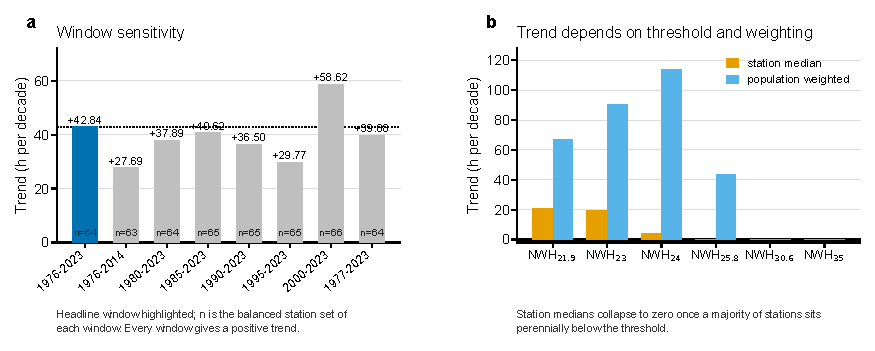
\includegraphics[width=\textwidth]{ExtendedDataFig1.pdf}
\caption{\textbf{Window robustness of the headline trend.} Theil--Sen trend of
$\mathrm{NWH}_{21.9}$ for eight start/end windows (1976--2023 headline); all windows are positive,
range $+27.69$ to $+58.62$\,h per decade.}
\label{fig:ed1}
\end{figure}

\begin{figure}[htbp]
\centering
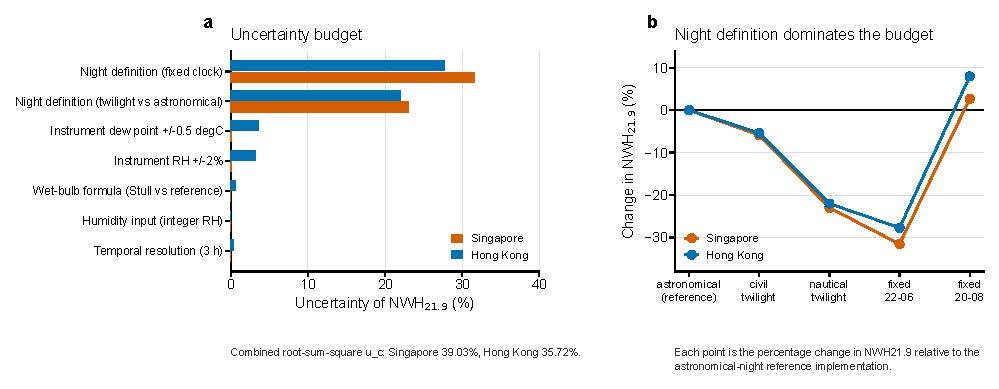
\includegraphics[width=\textwidth]{ExtendedDataFig2.pdf}
\caption{\textbf{Implementation uncertainty budget.} Component-wise and combined (root-sum-square)
relative uncertainty of the metric from a reference re-implementation at Hong Kong
($u_c=35.72\%$) and Singapore ($u_c=39.03\%$); the night definition dominates (22--32\%), wet-bulb
formula choice contributes $<0.6\%$.}
\label{fig:ed2}
\end{figure}

\begin{figure}[htbp]
\centering
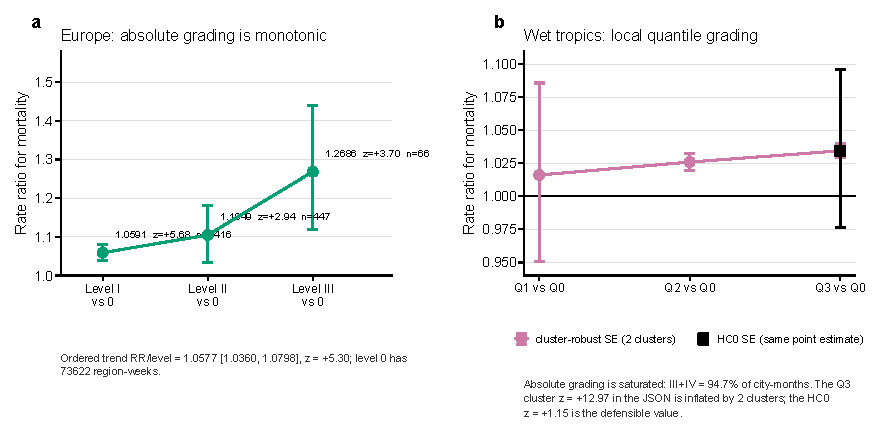
\includegraphics[width=\textwidth]{ExtendedDataFig3.pdf}
\caption{\textbf{Graded scale validation.} \textbf{a}, Mortality by graded level in Europe
(225 regions, 77,551 region-weeks): I $1.0591$ $[1.0384,1.0803]$, II $1.1049$ $[1.0338,1.1810]$,
III $1.2686$ $[1.1183,1.4391]$; monotone trend $1.0577$ per level, $z=+5.30$. \textbf{b}, Local
quantile grading in the wet tropics: with only two cities, cluster-robust SEs are unreliable and
HC0 intervals are reported alongside (Q3 HC0 CI $[0.9763,1.0962]$).}
\label{fig:ed3}
\end{figure}

\begin{figure}[htbp]
\centering
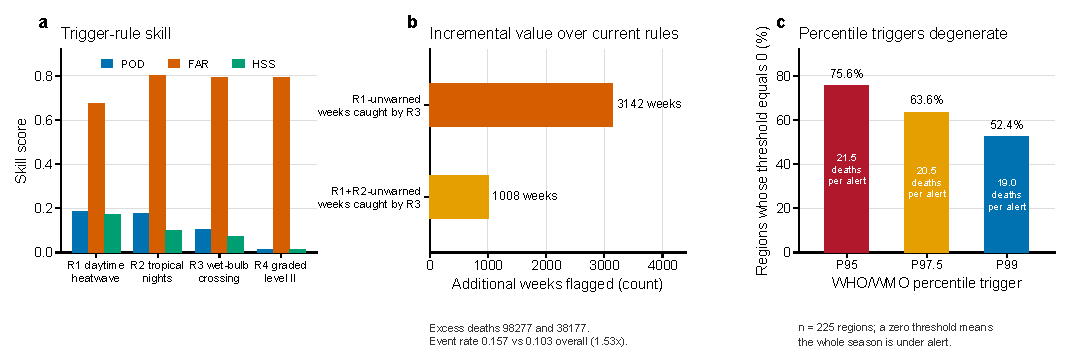
\includegraphics[width=\textwidth]{ExtendedDataFig4.pdf}
\caption{\textbf{Warning-skill evaluation and the percentile-trigger failure.} \textbf{a}, POD,
FAR and Heidke skill for four triggers; the nocturnal trigger alone (POD $0.102$) is below the
current daytime rule ($0.184$) and is positioned as an add-on. \textbf{b}, Incremental value:
3,142 weeks flagged only by the nocturnal trigger, event rate $1.53\times$ the panel average.
\textbf{c}, Zero-inflation failure of the WMO/WHO percentile default: the P95 (P97.5, P99)
warm-season $\mathrm{NWH}_{21.9}$ threshold equals zero in $75.6\%$ ($63.6\%$, $52.4\%$) of
European regions.}
\label{fig:ed4}
\end{figure}

\begin{figure}[htbp]
\centering
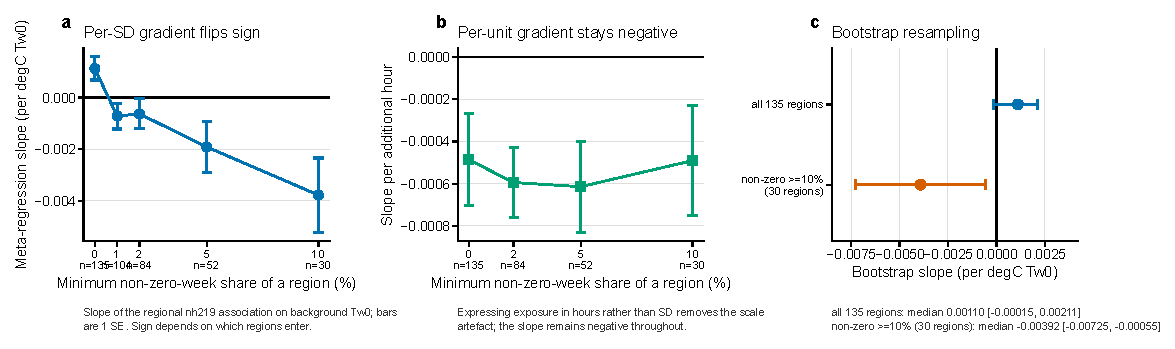
\includegraphics[width=\textwidth]{ExtendedDataFig5.pdf}
\caption{\textbf{Exposure--response gradient robustness.} Meta-regression of regional slopes on
background nocturnal $T_\mathrm{w}$: the unrestricted all-region slope is positive
($+0.00113$ per SD) but is driven by zero-variance regions; restricted to regions with non-zero
exposure in $\geq10\%$ of weeks the slope is negative ($-0.00377$); per-unit slopes are negative
throughout. Bootstrap intervals shown.}
\label{fig:ed5}
\end{figure}

\begin{figure}[htbp]
\centering
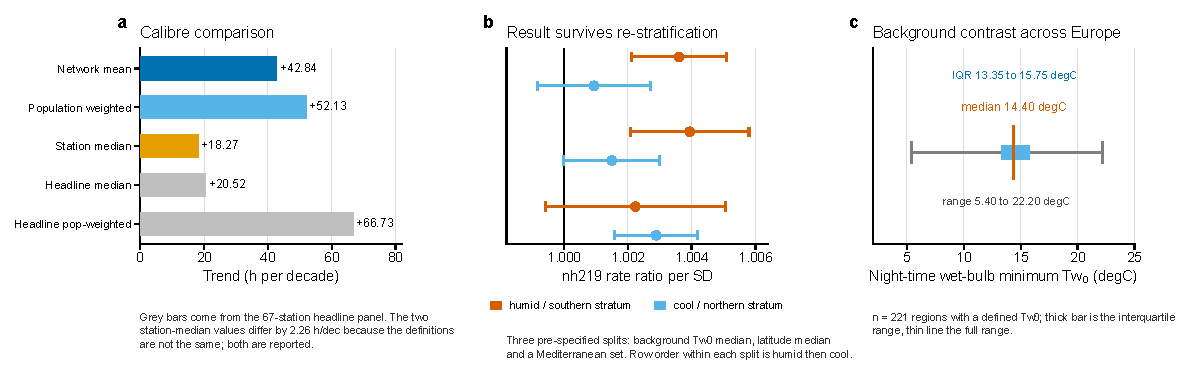
\includegraphics[width=\textwidth]{ExtendedDataFig6.pdf}
\caption{\textbf{Calibre and stratification robustness.} \textbf{a}, Two station-median
constructions of the headline trend (20.52 vs 18.27\,h per decade) are plotted side by side as
different estimators. \textbf{b}, The south--north contrast is stable across three stratification
schemes (background $T_\mathrm{w}$, latitude, Mediterranean): humid/southern strata 1.0036--1.0022
per SD versus cool/northern 1.0009--1.0015. \textbf{c}, Distribution of background warm-season
hottest-night wet-bulb minima across 221 regions (median 14.40\,\dd{}, IQR 13.35--15.75\,\dd{}).}
\label{fig:ed6}
\end{figure}

\clearpage

% ---------------------------------------------------------------------
% ed_table1.tex — Extended Data Table 1: complete frozen-results register
% (rows transcribed from tables/main_results_table.csv, formatting fixed)
% ---------------------------------------------------------------------
\begin{table}[p]
\centering
\scriptsize
\caption{\textbf{Complete register of frozen results, samples, specifications and status.}
Every numeric cell traces to a hash-verified artefact (see figures\_manifest.csv). Rows R1--R6 are
retracted, excluded or corrected items that are never presented as positive results.}
\label{tab:edtable1}
\begin{tabular}{rllp{2.6cm}p{4.6cm}l}
\toprule
\# & Fig. & Quantity & Sample & Effect (95\% CI unless stated) & Status \\
\midrule
1 & Fig1a & NWH21.9 trend, 1976--2023 & 64 stations, $\geq$90\% coverage, network equal-weighted & $+42.84$\,h per decade; baseline 1,546\,h\,yr$^{-1}$ & Primary \\
2 & Fig1b & Zero-inflation by threshold & 176 stations screened, 67 retained & NWH21.9: 17.7\% zero station-years, ratio 1.22$\times$; NWH35: 99.9\% zero & Limitation \\
3 & Fig1c & Aggregation sensitivity & identical 1976--2023 station set & $+42.84$ / $+52.13$ / $+18.27$\,h per decade & Sensitivity \\
4 & Fig2a & Moisture vs warming decomposition & 72 stations, counterfactuals A/B/C/D & moisture $+17.31$\,h/dec ($+105\%$); warming $+8.60$ ($+52\%$); interaction 0.00 & Primary \\
5 & Fig2b & Fingerprint ALL scaling factor & tropics + subtropics, 1976--2014; piControl $n=67$ segments & single $+0.429\pm0.148$; two-signal $+0.348$ (90\% CI $+0.072$ to $+0.624$) & Primary \\
6 & Fig2c & Observed vs modelled trends & 67 stations; 4 CMIP6 models & tropics obs $+50.30$ vs models $+103.08$ (S/N 3.08); subtropics $+15.48$ vs $+54.89$ (1.36) & Supporting \\
7 & Fig3a & Mortality, crossing 21.9\,\dd{} (any219) & 136 regions, 77,551 region-weeks & RR $=1.0181$ $[1.0104,1.0258]$, $z=+4.62$, $I^2=78.2\%$; AF $=1.77\%$ $[1.02,2.52]$ & Primary \\
8 & Fig3a & $+$ dry-bulb tropical-night control & 136 regions, joint binary model & any219 RR $=1.0292$ $[1.0212,1.0373]$, $z=+7.21$; dry-bulb RR $=1.0368$ $[1.0320,1.0416]$ & Identification \\
9 & Fig3b & Continuous specification & 135 regions, non-zero variance & RR per SD $=1.0033$ $[1.0020,1.0045]$, $z=+5.24$ & Sensitivity \\
10 & Fig3b & Strict whole-night definition & 30 regions with such events & RR $=1.0043$ $[0.9876,1.0212]$, $z=+0.50$ & Low power \\
11 & Fig3c & Dose--response bins & 64 regions, graded weekly exposure & 0--2\,h $1.0156$ $[1.0069,1.0243]$; 2--6\,h $1.0153$; 6--20\,h $1.0220$; $>$20\,h $0.9950$ $[0.9691,1.0216]$ & Step response \\
12 & Fig3d & South vs north Europe & south 101 / north 35 regions & south $1.0036$ $[1.0021,1.0051]$; north $1.0009$ $[0.9992,1.0027]$; contrast $z=+2.26$ ($p=0.024$) & Supporting \\
13 & Fig4a & Wet-tropics association (NWH25) & HK 132; SG 264 months & HK $1.0140$ ($z=+2.31$); SG $1.0073$ ($z=+1.69$); meta (orthogonalised) $1.0030$ $[1.0009,1.0051]$, $I^2=0\%$ & Replication \\
14 & Fig4b & Threshold saturation, Singapore & 300 months, 2001--2025 & 21.9\,\dd{} fraction 1.000; 24.0 0.981; 25.0 0.672; 25.8 0.098 & Limitation \\
15 & Fig4c & Re-thresholded models, Singapore & monthly panel, $n=300$ & NWH25.0 $1.0122$ ($z=+2.03$); NWH25.8 $1.0060$ ($z=+0.89$); NWH21.9 $1.0292$ ($z=+8.61$) REJECTED & Artefact + result \\
16 & Fig4d & Minimum detectable effect & HK 132; SG 264 months & HK $1.05\%$ per \dd{}; SG $2.46\%$ per \dd{} (ratio $2.33\times$) & Power limitation \\
17 & Fig5a & Extent vs intensity decoupling & 135 regions, 2000--2024 & population $+26\%$, regions $+29\%$, NWH $+47\%$; intensity-based scaling overstates $1.78\times$ & Primary \\
18 & Fig5b & Newly exposed population & 135 regions, 499 million & SSP2-4.5 end-century $+78$\,M (unscaled 166); SSP5-8.5 $+146$\,M (unscaled 237) & Primary \\
19 & Fig5c & Exposure response per $+1$\,\dd & same sample, calibrated & $70.0$\,M (pooled) / $42.3$\,M (fixed effects) & Primary \\
20 & ED2a & Implementation uncertainty budget & reference re-implementation, two cities & $u_c=39.03\%$ (SG), $35.72\%$ (HK); night definition dominates & Sensitivity \\
21 & ED3a & Graded scale, Europe & 225 regions, 77,551 region-weeks & I $1.0591$ $[1.0384,1.0803]$; II $1.1049$; III $1.2686$; trend $1.0577$/level & Monotonicity \\
22 & ED3b & Local quantile grading, tropics & two cities, 300 city-months & Q2 $1.0260$; Q3 $1.0345$ with 2-cluster caveat; HC0 CI for Q3 $[0.9763,1.0962]$ & Caveated \\
23 & ED4a & Warning trigger skill (R1--R4) & 77,551 region-weeks & R3 POD $=0.102$ below R1 POD $=0.184$; positioned as add-on & Supporting \\
24 & ED4b & Incremental nocturnal value & same panel & 3,142 weeks (98,277 deaths); event rate 0.157 vs 0.103 ($1.53\times$) & Supporting \\
25 & ED4c & WHO/WMO percentile-trigger failure & 225 regions; P95/P97.5/P99 & P95 $=0$ in 75.6\% of regions (63.6\%, 52.4\%); capture 21.5/20.5/19.0 deaths per alert & Guidance limit \\
26 & ED5 & Gradient robustness & 135 estimable regions of 225 & slope $+0.00113$ (all) vs $-0.00377$ (non-zero $\geq10\%$); per-unit slope negative & Sensitivity \\
27 & ED6b & Three stratification schemes & 225 regions, 77,551 region-weeks & humid/southern 1.0036/1.0039/1.0022; cool/northern 1.0009/1.0015/1.0009 & Supporting \\
28 & ED6c & Background humid-heat contrast & 221 regions with defined $T_{w0}$ & median 14.40\,\dd{}, IQR 13.35--15.75\,\dd{}, range 5.40--22.20\,\dd{} & Supporting \\
29 & T1 & Window sensitivity range & balanced sets per window & $+27.69$ to $+58.62$\,h per decade across eight windows & Sensitivity \\
30 & T1 & Moisture share, alternative calibres & same 72 stations & V: moisture $+19.45$ ($+118\%$), warming $+7.21$ ($+44\%$); L: $+6.70$ ($+41\%$), 0.00 & Sensitivity \\
31 & T1 & Band-resolved decomposition & 34 subtropical + 34 tropical stations & subtropics moisture $+48.88$, warming $+15.62$\,h/dec; tropics $+4.49$, $+1.51$ & Supporting \\
32 & T1 & Independent humidity attribution & 67 stations & temperature $+0.62$ (4\%), moisture $+6.70$ (39\%), interaction $+9.83$ (57\%) & Sensitivity \\
33 & T1 & Implementation uncertainty & HK + SG re-implementation & $u_c=35.72\%$ (HK), $39.03\%$ (SG) & Limitation \\
34 & T1 & Absolute grading, wet tropics & 300 city-months & levels III+IV occupy 94.7\% of city-months; level 0 absent & Limitation \\
\midrule
R1 & -- & First-crossing hazard ratio & 64-region cohort, 37 crossings & HR $=0.863$ NOT REPORTED: risk set cools $-2.50$\,\dd{} (frailty depletion) & Retracted \\
R2 & -- & WHO-style annual panel effect & outside frozen artefact set & not quantified; annual aggregation dilutes the nocturnal signal & Excluded \\
R3 & -- & Singapore NWH21.9 model & monthly panel, $n=300$ & RR/SD $=1.0292$ $[1.0225,1.0359]$, $z=+8.61$; exposure saturated (fraction 1.000) & Rejected artefact \\
R4 & -- & Printed heterogeneity statistic & 136 regions & frozen JSON $I^2=78.2\%$; earlier print showed 1\% (formatting bug) & Corrected \\
R5 & -- & Local-quartile Q3 cluster $z$ & 300 city-months, 2 cities & cluster $z=+12.97$ inflated (2 clusters); HC0 CI $[0.9763,1.0962]$ & Corrected \\
R6 & -- & Extent-versus-intensity direction & 135 regions & intensity $+47\%$ is FASTER than extent $+26\%$; earlier draft reversed & Corrected \\
\bottomrule
\end{tabular}
\end{table}
\clearpage


\end{document}
